\documentclass[12pt]{article}
\usepackage{algorithm2e}
\usepackage{amscd}
\usepackage{amsfonts}
\usepackage{amsmath}
\usepackage{amssymb}
\usepackage{amsthm}
\usepackage{authblk}
\usepackage[english]{babel}
\usepackage{bm}
\usepackage{caption}
\usepackage{color}
\usepackage{float}
\usepackage[perpage, symbol*]{footmisc}
\usepackage{graphicx}
\usepackage{hyperref}
\usepackage{enumerate}
\usepackage{mathrsfs}
\usepackage{natbib}
\usepackage{setspace}
\usepackage{subcaption}
\usepackage{tikz}
\usepackage{url}

\newcommand{\blind}{1}
\graphicspath{{figures/}}

\addtolength{\oddsidemargin}{-.5in}%
\addtolength{\evensidemargin}{-1in}%
\addtolength{\textwidth}{1in}%
\addtolength{\textheight}{1.7in}%
\addtolength{\topmargin}{-1in}%

\pdfminorversion=4

\DeclareMathOperator*{\argmax}{arg\,max}
\DeclareMathOperator*{\argmin}{arg\,min}
\newcommand{\T}{\intercal}

\theoremstyle{definition}
\newtheorem{definition}{Definition}
\newtheorem{theorem}{Theorem}

\setcitestyle{aysep={}}

\begin{document}

\def\spacingset#1{\renewcommand{\baselinestretch}%
{#1}\small\normalsize} \spacingset{1}


%%%%%%%%%%%%%%%%%%%%%%%%%%%%%%%%%%%%%%%%%%%%%%%%%%%%%%%%%%%%%%%%%%%%%%%%%%%%%%

\if1\blind
{
  \title{\bf A Principal Manifold-based Framework for Comparisons of Group-Level Manifold Estimates}
  \author{
    Robert Zielinski\hspace{.2cm}\\
    Department of Biostatistics, Brown University\\
    Kun Meng \\
    Division of Applied Mathematics, Brown University\\
    and \\
    Ani Eloyan \\
    Department of Biostatistics, Brown University\\
    for the Alzheimer's Disease Neuroimaging Initiative\thanks{Data used in preparation of this article were obtained from the Alzheimer's Disease Neuroimaging Initiative (ADNI) database (adni.loni.usc.edu). As such, the investigators within the ADNI contributed to the design and implementation of ADNI and/or provided data but did not participate in analysis or writing of this report. A complete listing of ADNI investigators can be found at \href{http://adni.loni.usc.edu/wp-content/uploads/how_to_apply/ADNI_Acknowledgement_List.pdf}{\texttt{http://adni.loni.usc.edu/wp-content/uploads/how\_to\_apply/ADNI\_Acknowledgement\_List.pdf}}}}
  \maketitle
} \fi

\if0\blind
{
  \bigskip
  \bigskip
  \bigskip
  \begin{center}
    {\LARGE\bf A Principal Manifold-based Framework for Comparisons of Group-Level Manifold Estimates}
\end{center}
  \medskip
} \fi

\bigskip
\begin{abstract}
Structural magnetic resonance imaging (MRI) data is frequently used to detect and monitor the progression of neurodegenerative conditions, such as Alzheimer's disease (AD). While 
\end{abstract}

\noindent%
{\it Keywords:}  Alzheimer's disease, smoothing spline, magnetic resonance imaging
\vfill

\newpage
\spacingset{1.9}
\section{Introduction} \label{s:hpme_intro}

Neurodegenerative diseases such as Alzheimer's disease (AD) and Parkinson's disease are highly complex, chronic conditions that exhibit substantial heterogeneity between patients. To enable researchers to identify potential biomarkers of progression for these conditions, large multi-site longitudinal observational studies have been conducted that collect information from a wide range of participants over long durations across several modalities, including neuroimaging (\cite{muellerWaysEarlyDiagnosis2005}, \cite{marekParkinsonProgressionMarker2011}). Neuroimaging data in particular have been shown to be sensitive to developments in the early stages of disease progression, often before diagnosis occurs (\cite{jackHypotheticalModelDynamic2010}).

While observations from neuroimaging data are typically high-dimensional, it is commonly assumed that the data lie along a low-dimensional manifold. Under this assumption, manifold learning algorithms can be used to recover this underlying manifold and parameterize the high-dimensional input data in the learned low-dimensional space. Most commonly-used manifold learning algorithms, including Isomap (\cite{tenenbaumGlobalGeometricFramework2000}), Locally Linear Embedding (\cite{roweisNonlinearDimensionalityReduction2000}), Laplacian Eigenmaps (\cite{belkinLaplacianEigenmapsDimensionality2003}), and Diffusion Maps (\cite{coifmanDiffusionMaps2006}) construct a graph of similarities between observations, which is then used to determine the structure of the manifold. \cite{mengPrincipalManifoldEstimation2021} present an alternative principal manifold framework for manifold estimation which extends to higher dimensions the principal curve framework introduced by \cite{hastiePrincipalCurves1989}, in which principal curves are defined as one-dimensional curves that pass through the middle of a high-dimensional dataset. 

In neuroimaging settings, manifold learning algorithms are most often applied at the population level, with vectorized image intensities being used as the input data. \cite{yueParameterizationWhiteMatter2016} used manifold learning to estimate a low-dimensional parameterization of the corpus callosum at the individual level. However, in many cases, the outcome of interest is framed as a comparison between different groups of individuals (e.g. treatment groups in a clinical trial). This goal is particularly relevant in the case of the complex neurodegenerative conditions mentioned above, where the high degree of heterogeneity in patient experiences has led to attempts to identify subgroups of patients based on a range of criteria such as symptom expression, onset, or rate of progression (\cite{ferreiraBiologicalSubtypesAlzheimer2020}, \cite{venutoPredictingAmbulatoryCapacity}). Fundamentally, if a low dimensional manifold is thought to effectively represent data related to the patient experience of a neurodegenerative condition, and the experience of that condition differs by group, then the low-dimensional representation of that experience should also differ by group.

A method to accurately and efficiently estimate the manifolds underlying data at the group level must take advantage of the grouped structure of observations. To develop an estimate of the manifold underlying the hippocampi of participants in the Alzheimer's Disease Neuroimaging Initiative (ADNI) study, it is necessary to recognize the basic nesting structure of the data, in which brain images are nested within participants belong to a latent disease subgroup where patients tend to have more related symptom experiences or underlying physiological developments. These subgroups are in turn nested within study groups based on Alzheimer's disease status, which are finally nested within the greater study population. In this paper, we develop a manifold learning approach that appropriately accounts for this hierarchical structure when estimating the manifolds underlying such data. We further propose an approach for estimation of the underlying manifold at each level of the hierarchy, allowing for statistical testing of differences between those low-dimensional manifolds.

There have been attempts to address hierarchical structure in manifold learning problems. \cite{bhatiaHierarchicalManifoldLearning2012} introduced a modification of Laplacian eigenmaps to estimate manifolds from recursively subdivided regions of medical images while enforcing similar alignment of the manifolds estimated from related regions. \cite{freicheCharacterizingMyocardialIschemia2022} built on this approach to incorporate multiple imaging modalities and automate the tuning of the algorithm's hyperparameters. \cite{gaoHierarchicalManifoldLearning2019} proposed a two-step diffusion maps method for hierarchical data with variation over several domains, where diffusion maps is applied first to reduce the dimension of the images for each individual, resulting in individual-specific manifold estimates, then diffusion maps is applied again on the concatenated parameterizations to reduce over the individuals, thus estimating a group-level manifold. This approach allows the first step of dimension reduction to capture the most important qualities of each image separately before reducing across subjects, but the two step procedure does not ensure that the manifold estimated at the individual level is structurally related to the manifold estimated at the group level, posing problems for the interpretability of the embedding mappings and comparisons of manifolds between levels.

\cite{guerreroGroupconstrainedManifoldLearning2017} noted that, when using graph-based embedding methods to estimate a manifold from population data, the grouping behavior of observations recorded longitudinally from the same individual adversely impacted the creation of the neighborhood graph between data points. The authors proposed a constraint specifying that a given observation's collection of nearest neighbors may include at most one point from each individual or other given grouping. This encourages a more even representation of the entire space of observations in the neighborhood graph, and may be applied to any manifold learning algorithm that features a neighborhood graph to represent proximities between observations. However, it simply mitigates the effects of the nesting structure on a population-level manifold estimate rather than enabling a detailed comparison of manifold estimates for each group.

In this work, we build on the principal manifold estimation (PME) algorithm introduced by \cite{mengPrincipalManifoldEstimation2021}, which uses an iterative procedure to specify an embedding mapping from the low-dimensional manifold to a high-dimensional space that takes the form of a smoothing spline. Drawing from literature in hierarchical and additive models, we replace the smoothing spline in the PME algorithm with an additive smoothing spline model (\cite{gelmanDataAnalysisUsing2007}, \cite{hastieGeneralizedAdditiveModels1990}, \cite{gelmanBayesianDataAnalysis2014}). While the specific model structure may change to meet the needs of the application, \cite{brumbackSmoothingSplineModels1998} and \cite{schulamFrameworkIndividualizingPredictions2015a} provide examples of additive spline models used for different applications. The use of additive spline models ultimately yields a nonlinear dimension reduction algorithm that takes advantage of a statistically principled model to address nesting structures of the input data. As it is based on the PME framework, the algorithm outputs an explicit representation of the embedding function, making it possible to both generate new data in high-dimensional space using low-dimensional parameters and map new input data to the estimated manifold. Smoothing spline analysis of variance may allow the statistical comparison of the estimated manifolds between groups or individuals (\cite{wangMixedEffectsSmoothing1998}).

The following sections are organized as follows. Section \ref{s:methods} specifies an additive smoothing spline model for use in the analysis of neuroimaging data from the ADNI study, and provides a comprehensive description of the hierarchical PME algorithm developed in this paper. Section \ref{s:hpme_mnist_simulation} applies this method to the MNIST dataset of handwritten digits, and compares the results to those produced using PME. The performance of the two approaches is then compared when they are applied to a series of simulated datasets of varying complexities. Section \ref{s:hpme_adni} discusses proposed work, which will demonstrate how the model specified in Section \ref{s:methods} may be used for the estimation of a manifold underlying the surfaces of subcortical structures of participants of the ADNI dataset. This will be followed by a concluding discussion of the proposed algorithm and opportunities for further study.

\section{Methods}\label{s:methods}

\subsection{Additive Smoothing Spline Model}

We begin this section with a brief review of additive models. Consider a regression scenario where the dependent variable $\mathbf{y} = \left(y_1, \dots, y_n\right)^{T}$ is thought to be associated with independent covariate vectors $\mathbf{x}_i = \left(x_{i1}, \dots, x_{ip}\right)$, for $i = 1, \dots, n$, with $n$ representing the number of observations. In this situation, the standard multiple linear regression model assumes that the dependence of $y_i$ on $\mathbf{x}_i$ takes the linear form
\[%
  y_i = \alpha + x_{i1}\beta_1 + \dots + x_{ip}\beta_p + \epsilon_i
,\]%
where $\epsilon$ has mean 0 and variance $\sigma^2$. Additive models are a direct extension of this model, where the additive structure of the model is retained, but the assumption of linearity is discarded. A simple additive model takes the form
\begin{equation}
  y_i = \alpha + \sum_{j=1}^{p}f_j(X_{ij}) + \epsilon_i, \label{eq:1}
\end{equation}
where again $\epsilon_i$ has mean 0 and variance $\sigma^2$, however for each $j$, $f_j$ represents an arbitrary function commonly assumed to be smooth. While the functions in model \ref{eq:1} only take as parameters the value of one covariate, with each covariate being represented in the model once, this does not need to be the case, as functions specifying interactions between covariates may also be included. The structure of additive models seeks to balance benefits of interpretability found in linear regression models with the flexibility of nonlinear, and frequently, nonparametric functional forms. Further information can be found in \cite{hastieGeneralizedAdditiveModels1990}.

With this background in place, we turn to the motivating example of analyzing the subcortical surfaces of ADNI participants using MR images, with a focus on the hippocampus, although the framework can be applied to modeling other structures in the brain. ADNI is a longitudinal observational study, where several imaging modalities are used to record brain images from participants over time. Participants can generally be considered to belong to three groups based on cognitive state: elderly healthy controls, those displaying symptoms of mild cognitive impairment, and those diagnosed with AD. In practice, participants may transition between these categorizations as their symptoms progress. However, because patients may be diagnosed with AD at different stages, accurately modeling these transitions is challenging and is beyond the scope of this manuscript. For simplicity, we use the groupings recorded at the time each participant was recruited to the study. 

Individual participants are typically scheduled for imaging at six month intervals, though variability exists in the recorded intervals. Also of note, the numbers of observations contributed by each participant varies, so groups may be unbalanced. We denote the number of groups under consideration using $G$, the number of individuals included in the study as $I$, the number of images available as $N$, and the number of observations available for the $j$th image as $Q_j$, with $j = 1, 2, \dots, N$. The individual to which the $j$th image belongs is denoted as $i(j)$, the group of the $i(j)$th individual is represented by $g(j)$, and we use $t_j$ to denote the time at which the $j$th image was recorded, with all times being relative to the $i(j)$th individual's baseline visit. This time benchmark may be changed to age, time from diagnosis, time from symptom onset, or any other measure of time, depending on the setting. Finally, we use $N_t$, $N_i$, and $N_g$ to denote the number of images available for time point $t$, individual $i$, and group $g$, respectively.

Within a segmented structural MRI, the voxels estimated to mark the surface of the hippocampus can be assumed to lie along a two-dimensional manifold that has been wrapped into the three-dimensional image space. More generally, we let $d$ denote the intrinsic dimension of the low-dimensional manifold, and $D$ represent the dimension of the high-dimensional input space. For the $j$th image with $j = 1, \dots, N$, we denote the $q$th voxel in the $D$-dimensional space as $\mathbf{x}_{jq} \in \mathbb{R}^{D}$, its associated $d$-dimensional parameterization as $\mathbf{y}_{jq} \in \mathbb{R}^{d}$, and its weight as $w_{jq}$. We use $\mathbf{x}_g$, $\mathbf{x}_i$, $\mathbf{x}_{j}$, and $\mathbf{x}_t$ to denote the input voxels from all images in the $g$th group, $i$th individual, $j$th image, and $t$th time point, respectively, and use similar notation for all other relevant terms.

The embedding function which maps from the $d$-dimensional manifold to $D$-dimensional ambient space is represented as $\psi(\mathbf{y}_{jq})$, which can be modeled as 
\begin{equation}
  \mathbf{x}_{jq} = \psi(\mathbf{y}_{jq}, t_j) = f_p(\mathbf{y}_{jq}, t_{j}) + f_{g(j)}(\mathbf{y}_{jq}, t_{j}) + f_{i(j)}(\mathbf{y}_{jq}, t_{j}) + f_j(\mathbf{y}_{jq}) + \epsilon_{jq}j. \label{eq:2}
\end{equation}
The embedding map $\psi(\mathbf{y})$ is associated with a projection index $\kappa_{\psi}(\mathbf{x}): \mathbb{R}^{D} \to \mathbb{R}^{d}$, which, informally, outputs the $d$-dimensional parameterization $\mathbf{y}$ that minimizes $\|\mathbf{x} - \psi(\mathbf{y})\|_{\mathbb{R}^{D}}$ and follows the generalized definition of projection indices given in \cite{mengPrincipalManifoldEstimation2021}.

Each function in this additive model represents a different level of nesting in the data, with $f_p(\mathbf{y}, t)$ estimating the embedding at the population level, and $f_g(\mathbf{y}, t)$, $f_i(\mathbf{y}, t)$, and $f_{j}(\mathbf{y})$ describing deviations from the population estimates specific to the group, individual, and image in question, respectively. As estimating longitudinal changes in the underlying manifold may be of interest, $f_p(\mathbf{y}, t)$, $f_g(\mathbf{y}, t)$ and $f_i(\mathbf{y}, t)$ are each denoted as varying-coefficient models, where the coefficients of each function are dependent on time (\cite{hastieVaryingCoefficientModels1993}). Thus, the model is capable of estimating separate longitudinal changes for population, group, and individual estimates. In cases where longitudinal changes are not of interest, each varying-coefficient model may be constrained to be held constant with respect to time. As the $j$th image is recorded at a single time point, $f_{j}(\mathbf{y}, t)$ may not be dependent on time. We specify $f_{j}(\mathbf{y})$ as a smoothing spline, while the functions $f_p(\mathbf{y}, t)$, $f_g(\mathbf{y}, t)$, and $f_i(\mathbf{y}, t)$ are each varying-coefficient smoothing spline models, estimated by using a smoothing spline to smooth over smoothing spline coefficients calculated at each time point available in the data. 

The smoothing spline functions $f(\mathbf{y})$ minimize 
\[%
  \mathcal{K}_{\lambda}(f) = \sum_{j=1}^{N}\sum_{q=1}^{Q_j}w_{jq}\|\mathbf{x}_{jq} - f(\mathbf{y}_{jq})\|^2_{\mathbb{R}^{d}} + \lambda\|\nabla^{\otimes 2}f\|^2_{L^2(\mathbb{R}^{d})}
,\]%
where $\nabla^{\otimes 2}f$ denotes the Hessian matrix of $f$, and $\lambda$ is a given parameter used to penalize curvature in $f$. Thus, $f(\mathbf{y})$ takes the form
\begin{equation}
  f_l(\mathbf{y}) = \sum_{j=1}^{N}\sum_{q=1}^{Q_j}s_{jq, l} \times \eta_{d}\left(\|\mathbf{y} - \mathbf{y}_{jq}\|\right) + \sum_{p = 1}^{d + 1}\alpha_{p, l} \times \phi_{p}(\mathbf{y}), \quad l = 1, 2, \dots, D, \label{eq:3}
\end{equation}
with $\phi_p(\mathbf{y})$ representing the basis of the linear space of polynomials on $\mathbb{R}^{d}$ with degree $\leq 1$ and $\eta_{d}(y) = y^{4-d}\log y$ when $\log y \neq 0$ and $d$ is even, $\eta_{d}(y) = 0$ when $\log y = 0$ and $d$ is even, and $\eta_{d}(y) = y^{4-d}$ when $d$ is odd. 

Without accounting for the additive structure of the model, and after concatenating all relevant values into $Q = \sum_{j=1}^{N}Q_{j}$-dimensional vectors of input values $\mathbf{y}$, weights $\mathbf{w}$, and outputs $\mathbf{x}$, we can estimate $f$ by obtaining the values of $s_l \in \mathbb{R}^{Q}$ and $\alpha_l \in \mathbb{R}^{d + 1}$ for $l = 1, \dots, D$ that minimize $\|\mathbf{W}^{\frac{1}{2}}\left(\mathbf{x}_{l} - \mathbf{E}s_l - \mathbf{R}\alpha_l\right)\|^2_{\mathbb{R}^{Q}} + \lambda\|\mathbf{E}^{\frac{1}{2}}s_l\|^2_{\mathbb{R}^{Q}}$ under the constraint that $\mathbf{R}^{T}s_l = 0$, where
\begin{itemize}
  \item $\mathbf{E} = (E_{qr})_{1 \leq q, r, \leq Q}$ is defined by $E_{qr} = \eta_{d}\left(\|\mathbf{y}_{q} - \mathbf{y}_{r}\|\right))$.
  \item $\mathbf{R} = \left(R_{mp}\right)_{1 \leq m \leq Q, \ 1 \leq p \leq d + 1}$ is defined by $R_{mp} = \phi_p(\mathbf{y}_{m})$.
  \item $\mathbf{W} = diag(w_{1}, \dots, w_{Q})$.
\end{itemize}

With $\upsilon_l$ representing Lagrange multipliers, the solutions for $s_l$ and $\alpha_l$ can be found by solving

\begin{equation}
   \left(\begin{array}{ccc}
    2\mathbf{EWE} + 2\lambda\mathbf{E} & 2\mathbf{EWR} & \mathbf{R} \\
    2\mathbf{R}^{T}\mathbf{WE} & 2\mathbf{R}^{T}\mathbf{WR} & \mathbf{0} \\
    \mathbf{R}^{T} & \mathbf{0} & \mathbf{0}
  \end{array}\right)\left(
  \begin{array}{c}
    s_l \\
    \alpha_l \\
    \upsilon_l
  \end{array}
  \right) = \left(
  \begin{array}{c}
    2\mathbf{EW}\mathbf{x}_l \\
    2\mathbf{R}^{T}\mathbf{W}\mathbf{x}_l \\
    \mathbf{0}
  \end{array}
  \right). \label{eq:4}
\end{equation}
The optimal value of $\lambda$ can be found using cross-validation, where with images being randomly split into $K$ folds, functions may be evaluated by the mean squared error, written as
\begin{equation}
  MSD(\lambda) = \frac{1}{K}\sum_{k=1}^{K}\frac{1}{N_u}\sum_{j=1}^{N_u}\frac{1}{Q_j}\sum_{q=1}^{Q_j}\|\mathbf{x}_{jq} - f_{\lambda}^{(k)}(\mathbf{y}_{jq})\|^2. \label{eq:5}
\end{equation}
Here, $f_{\lambda}^{(k)}(\mathbf{y})$ denotes the estimated spline function given tuning parameter $\lambda$ and with the data for the $k$th fold excluded.

The coefficients and tuning parameter that minimize $\mathcal{K}_{\lambda}(f)$ suffice for estimating $f_{j}(\mathbf{y})$, in which the coefficients are not time-varying. To reach estimates for the varying-coefficient models, equation \ref{eq:4} is solved using the data available at each time point within the relevant study level. To estimate $f_p(\mathbf{y}, t)$, we use $\left\{\mathbf{x}_t\right\}_{t=1}^T$ and $\left\{\mathbf{y}_t\right\}_{t=1}^T$, yielding fitted function $\left\{\hat{f}_t(\mathbf{y})\right\}_{t=1}^T$. Using the maximum and minimum values of $\mathbf{y}_t$ in each dimension, a new $d$-dimensional grid of $Q' = \text{max}\left(\left\{Q_{j}\right\}_{j = 1}^{N}\right)$ knots, $\left\{\mathbf{y'}_q\right\}_{q=1}^{Q'}$, is generated with the knots being evenly spread throughout the parameter space. These parameters serve as common knots that allow the spline coefficients to be compared across time points. They are then used to compute a new set of corresponding outcome values $\left\{\mathbf{x}'_t\right\}_{t=1}^{T}$. The spline functions are reestimated as $\left\{\hat{f}'_t\right\}_{t=1}^{T}$ using $\left\{\mathbf{x}'_t\right\}_{t=1}^{T}$ and $\mathbf{y}'$. These newly generated knots are weighted equally, so an unweighted smoothing spline model is used. Following \cite{greenSilverman1994}, we let

\begin{itemize}
  \item $\mathbf{E}' = \left(E'_{qr}\right)_{1 \leq q, r, \leq Q'}$ defined by $E'_{qr} = \eta_{d}\left(\|\mathbf{y}'_{q} - \mathbf{y}'_{r}\|\right)$.
  \item $\mathbf{R}' = \left(R'_{mp}\right)_{1 \leq m \leq Q', \ 1 \leq p \leq d + 1}$ is defined by $R'_{mp} = \phi_p(\mathbf{y'}_{m})$.
\end{itemize}

Then the coefficients that minimize $\left(\mathbf{x}'_t - \mathbf{E}'\mathbf{s}_t - \mathbf{R}'^{T}\mathbf{\alpha}_t\right)^{T}\left(\mathbf{x}'_t - \mathbf{E}'\mathbf{s}_t - \mathbf{R}'^{T}\mathbf{\alpha}_t\right) + \gamma\mathbf{s}_t^{T}\mathbf{E}'\mathbf{s}_t$ can be found by solving 
\begin{equation}
  \left(
  \begin{array}{cc}
    \mathbf{E}' + \lambda_{t}\mathbf{I} & \mathbf{R}'^{T} \\
    \mathbf{R}' & \mathbf{0}
  \end{array}
  \right)\left(
  \begin{array}{c}
    \mathbf{s}'_t \\
    \mathbf{\alpha}'_t
  \end{array}
  \right) = \left(
  \begin{array}{c}
    \mathbf{x}'_t \\
    \mathbf{0}
  \end{array}
  \right). \label{eq:6}
\end{equation}

The coefficients found at each time point $t$, $\mathbf{s'}_{t}$ and $\mathbf{\alpha'}_{t}$ are concatenated in matrix $\mathbf{\omega}_{t} = \left(\mathbf{s'}_{t}^T, \mathbf{\alpha'}_{t}^T\right)$. This coefficient matrix is then used as the output value in a cubic smoothing spline function using the time points as input values. This function takes the form

\[%
  g_{\gamma}(t) = \sum_{i=1}^{T}\delta_i\|t - t_i\|^{3} + \sum_{p=1}^{2}\tau_p \phi(t)_p
.\]%
We define matrix $\mathbf{A}$ as $\mathbf{A}_{qr} = \|t_q - t_r\|^{3}$, matrix $\mathbf{T}$ as $\mathbf{T}_{pr} = \phi_p(t_r)$, $\mathbf{\delta} = \left(\delta_1, \dots, \delta_T\right)^{T}$, and $\mathbf{\tau} = \left(\tau_1, \tau_2\right)^{T}$. Then, the coefficients of $g_{\gamma}(t)$, given a value of $\gamma$, can be found by solving
\begin{equation}
  \left(
  \begin{array}{cc}
    \mathbf{A} + \gamma\mathbf{I} & \mathbf{T}^{T} \\
    \mathbf{T} & \mathbf{0}
  \end{array}
  \right)\left(
  \begin{array}{c}
    \mathbf{\delta} \\
    \mathbf{\tau}
  \end{array}
  \right) = \left(
  \begin{array}{c}
    \mathbf{\omega} \\
    \mathbf{0}
  \end{array}
  \right). \label{eq:7}
\end{equation}

As with the tuning process for $\lambda$, the optimal value of $\gamma$ can be identified using cross-validation, with either leave-one-out or $k$-folds cross-validation being appropriate depending on the number of time points available. If using leave-one-out cross-validation, the mean squared error can be calculated as
\begin{equation}
  MSD(\gamma) = \frac{1}{T}\sum_{t=1}^{T}\frac{1}{N_t}\sum_{j=1}^{N_t}\frac{1}{Q_j}\sum_{q=1}^{Q_j}\|\mathbf{x}_{jq} - f_{\gamma}^{(t)}(\mathbf{y}_{jq}, t_j)\|^2. \label{eq:8}
\end{equation}
We then let $\hat{\gamma}$ be the value of $\gamma$ that minimizes $MSD(\gamma)$.

With a proper estimate of the $\hat{\gamma}$, we may denote the coefficients of $g(t)$ as $\Omega = \left(\delta^{T}, \tau^{T}\right)$, and those estimated by $g(t)$ as $\omega(t) = \left(\mathbf{s}_{\hat{\gamma}}(t)^{T}, \mathbf{\alpha}_{\hat{\gamma}}(t)^{T}\right)^{T}$. We use these coefficients in equation \ref{eq:3} in place of the constant coefficients. Therefore, the varying-coefficient models have the following outputs:
\begin{equation}
  f(\mathbf{y}, t) = \sum_{q=1}^{Q'}\mathbf{s}_{\hat{\gamma}, l}(t) \eta_{d}\left(\|\mathbf{y} - \mathbf{y'}_m\|\right) + \sum_{p=1}^{d + 1}\mathbf{\alpha}_{\hat{\gamma}, p, l}(t) \phi_p(\mathbf{y}), \quad l = 1, \dots, D. \label{eq:9}
\end{equation}
The fitting process for the varying-coefficient smoothing spline model is given formally as Algorithm \ref{alg:varying_spline}.

\SetKwComment{Comment}{/* }{ */}

\RestyleAlgo{ruled}
\LinesNumbered

\begin{algorithm}
\caption{Varying-Coefficient Smoothing Spline Model}\label{alg:varying_spline}
  \KwData{$D$-dimensional output values $\left\{\mathbf{x}_{jq}\right\}_{j = 1, q = 1}^{N, Q_{j}}$, $d$-dimensional input values $\left\{\mathbf{y}_{jq}\right\}_{j=1, q=1}^{N, Q_{j}}$, weights $\left\{w_{jq}\right\}_{j=1, q=1}^{N, Q_{j}}$, observation times $\left\{t_{j}\right\}_{j=1}^{N}$, candidate tuning parameters $\left\{\lambda_l\right\}_{l=1}^{L}$, $\left\{\gamma_p\right\}_{p=1}^{P}$, and number of cross-validation folds $K$.}
  \KwResult{Analytic formula of $\hat{f}(\mathbf{y}, t)$, coefficients $\Omega = \left(\mathbf{\delta}^{T}, \mathbf{\tau}^{T}\right)$, and optimal tuning parameter $\hat{\gamma}$.}

\For{$t = 1, 2, \dots, T$} {
  Set $U_t$ equal to the number of images included in the data at time $t$\;
  \For{$l = 1, 2, \dots, L$} {
    Solve equation \ref{eq:4} to estimate $f_{\lambda_l, t}(\mathbf{y})$ with inputs $\mathbf{x}_t$, $\mathbf{y}_t$, and $w_t$\;
    \For{$u = 1, 2, \dots, U_t$} {
      Solve equation \ref{eq:4} to estimate $f^{(-u)}_{\lambda_l, t}(\mathbf{y})$ with inputs $\mathbf{x}^{(-u)}_t$, $\mathbf{y}^{(-u)}_t$, $w^{(-u)}_t$\;
      Estimate $MSD(\lambda_{l})_u$ using equation \ref{eq:5}\;
    }
    Set $MSD(\lambda_l) = \frac{1}{U}\sum_{u=1}^{U}MSD(\lambda_l)_u$\;
  }
  $\hat{\lambda}_t = \arg \min_{\lambda} MSD(\lambda)$\;
  $f_t(\mathbf{y}) = f_{\hat{\lambda}_t}(\mathbf{y})$\;
}

  Let $Q' = \max(Q_{j})$, $\left\{\mathbf{y}'_{q}\right\}_{q=1}^{Q'}$ be a grid spanning the range of values of $\left\{\mathbf{y}_{jq}\right\}_{j=1, q=1}^{N, Q_j}$\;
  \For{$t = 1, 2, \dots, T$} {
    Compute $\left\{\mathbf{x'}_{q, t}\right\}_{q=1}^{Q'} = \left\{f_t(\mathbf{y'}_q)\right\}_{q=1}^{Q'}$\;
    Solve equation \ref{eq:6} to compute $\mathbf{s'}_t$ and $\mathbf{\alpha'}_t$\;
    Set $\mathbf{\omega}_t = \left[\mathbf{s'}_t^{T}, \mathbf{\alpha'}_t^{T}\right]$\;
  }
  \For{$p = 1, 2, \dots, P$} {
    Compute $g_{\gamma_p}(t)$ by solving equation \ref{eq:7}\;
    \For{$t = 1, 2, \dots, T$} {
      Compute $g_{\gamma_p}^{(t)}$ by solving \ref{eq:7}\;
    }
    Estimate $MSD(\gamma_p)$ using \ref{eq:8}\;
  }
  $\hat{\gamma} = \arg \min_{\gamma} MSD(\gamma)$\;
  $\hat{f}(\mathbf{y}, t) = f_{\hat{\gamma}}(\mathbf{y}, t)$, where the form of $\hat{f}(\mathbf{y}, t)$ is given in \ref{eq:9}.
\end{algorithm}

While the procedure outlined in Algorithm \ref{alg:varying_spline} yields an appropriate estimator when working with unnested data, this approach must be adapted to work within the additive model structure of model \ref{eq:2}. As discussed in \cite{hastieGeneralizedAdditiveModels1990}, the additive model $\psi(\mathbf{y}, t)$ can be estimated using a backfitting procedure, which uses the model's additive nature to iteratively fit each distinct smoothing spline function until convergence. Specifically, we use the fact that, under the model,

\[%
  f_p(\mathbf{y}_{jq}, t_{j}) = E\left[\mathbf{x}_{jq} - f_{g(j)}(\mathbf{y}_{jq}, t_{j}) - f_{i(j)}(\mathbf{y}_{jq}, t_{j}) - f_{j}(\mathbf{y}_{jq})\right]
,\]%
with a similar result holding for each of the smooth functions making up the additive model. The model in its entirety is considered to have converged when the maximum of the distances between the coefficients of functions estimated for the same element in consecutive steps is below a given threshold. Details of the backfitting algorithm to fit the proposed model is given in Algorithm \ref{alg:backfitting}.

\begin{algorithm}
\footnotesize
\caption{Backfitting Algorithm for Additive Spline Model}\label{alg:backfitting}
  \KwData{$D$-dimensional output values $\left\{\mathbf{x}_{jq}\right\}_{j=1, q=1}^{N, Q_{j}}$, $d$-dimensional input values $\left\{\mathbf{y}_{jq}\right\}_{j=1, q=1}^{N, Q_{j}}$, observation times $\left\{t_{j}\right\}_{j=1}^{N}$, weights $\left\{w_{jq}\right\}_{j=1, q=1}^{N, Q_j}$, group and individual indicator values $\left\{g(j)\right\}_{j=1}^{N}$ and $\left\{i(j)\right\}_{j=1}^{N}$, candidate tuning parameters $\left\{\lambda_l\right\}_{l=1}^{L}$ and $\left\{\gamma_p\right\}_{p=1}^{P}$, $\epsilon$ and $K$.}
  \KwResult{Analytic formulas of $\hat{f}_p$, $\left\{\hat{f}_g\right\}_{g=1}^{G}, \left\{\hat{f}_i\right\}_{i=1}^{I}$, and $\left\{\hat{f}_{j}\right\}_{j=1}^{N}$.}

  Estimate $f_{p}^{(0)}(\mathbf{y}, t)$ and $\Omega_{p}^{(0)}$ using Algorithm \ref{alg:varying_spline} with inputs $\left\{\mathbf{x}_{jq}\right\}_{j=1, q=1}^{N, Q_j}$, $\left\{\mathbf{y}_{jq}\right\}_{j=1, q=1}^{N, Q_j}$, $\left\{w_{jq}\right\}_{j=1, q=1}^{N, Q_j}$, $\left\{t_{j}\right\}_{j=1}^{N}$, $\left\{\lambda_l\right\}_{l=1}^{L}$, $\left\{\gamma_p\right\}_{p=1}^{P}$, and $K$\;
  \For{$g = 1, 2, \dots, G$} {
    Estimate $f_{g}^{(0)}(\mathbf{y}, t)$ and $\Omega_{g}^{(0)}$ using Algorithm \ref{alg:varying_spline} with inputs $\left\{\mathbf{x}_{jq} - f_{p}^{(0)}(\mathbf{y}_{jq}, t_j)\right\}_{j=1, q=1}^{N_g, Q_j}$, $\left\{\mathbf{y}_{jq}\right\}_{j=1, q=1}^{N_g, Q_j}$, $\left\{w_{jq}\right\}_{j=1, q=1}^{N_g, Q_j}$, $\left\{t_j\right\}_{j=1}^{N_g}$, $\left\{\lambda_l\right\}_{l=1}^{L}$, $\left\{\gamma_p\right\}_{p=1}^{P}$, $K$\;
  }
  \For{$i = 1, 2, \dots, I$} {
    Estimate $f_{i}^{(0)}(\mathbf{y}, t)$ and $\Omega_{i}^{(0)}$ using Algorithm \ref{alg:varying_spline} with inputs $\left\{\mathbf{x}_{jq} - f_{p}^{(0)}(\mathbf{y}_{jq}, t_j) - f_{g(j)}^{(0)}(\mathbf{y}_{jq}, t_j)\right\}_{j=1, q=1}^{N_i, Q_j}$, $\left\{\mathbf{y}_{jq}\right\}_{j=1, q=1}^{N_i, Q_j}$, $\left\{w_{jq}\right\}_{j=1, q=1}^{N_i, Q_j}$, $\left\{t_j\right\}_{j=1}^{N_i}$, $\left\{\lambda_l\right\}_{l=1}^{L}$, $\left\{\gamma_p\right\}_{p=1}^{P}$, and $K$\;
  }
  \For{$j = 1, 2, \dots, N$} {
    Estimate $f_{j}^{(0)}(\mathbf{y})$ and $\omega_{j}^{(0)}$ by solving \ref{eq:4} with inputs $\left\{\mathbf{x}_{jq} - f_{p}^{(0)}(\mathbf{y}_{jq}, t_j) - f_{g(j)}^{(0)}(\mathbf{y}_{jq}, t_j) - f_{i(j)}^{(0)}(\mathbf{y}_{jq}, t_j)\right\}_{q=1}^{Q_j}$, $\left\{\mathbf{y}_{jq}\right\}_{q=1}^{Q_j}$, $\left\{w_{jq}\right\}_{q = 1}^{Q_j}$, $\left\{\lambda_l\right\}_{l=1}^{L}$, $K$\;
  }
  $n \gets 0$\;
  \While{$\max\left(\|\Omega_p^{(n)} - \Omega_{p}^{(n-1)}\|, \left\{\|\Omega_{g}^{(n)} - \Omega_{g}^{(n-1)}\|\right\}_{g=1}^{G}, \left\{\|\Omega_{i}^{(n)} - \Omega_{i}^{(n-1)}\|\right\}_{i=1}^{I}, \left\{\|\omega_{j}^{(n)} - \omega_{j}^{(n-1)}\|\right\}_{j=1}^{N}\right) \geq \epsilon$} {
    Estimate $f_{p}^{(n+1)}(\mathbf{y}, t)$ and $\Omega_{p}^{(n+1)}$ using Algorithm \ref{alg:varying_spline} with inputs $\left\{\mathbf{x}_{jq} - f_{g(j)}^{(n)}(\mathbf{y}_{jq}, t_j) - f_{i(j)}^{(n)}(\mathbf{y}_{jq}, t_j) - f_j^{(n)}(\mathbf{y}_{jq})\right\}_{j=1, q=1}^{N, Q_j}$, $\left\{\mathbf{y}_{jq}\right\}_{j=1, q=1}^{N, Q_j}$, $\left\{w_{jq}\right\}_{j=1, q=1}^{N, Q_j}$, $\left\{t_{j}\right\}_{j=1}^{N}$, $\left\{\lambda_l\right\}_{l=1}^{L}$, $\left\{\gamma_p\right\}_{p=1}^{P}$, and $K$\;
    \For{$g = 1, 2, \dots, G$} {
      Estimate $f_{g}^{(n+1)}(\mathbf{y}, t)$ and $\Omega_{g}^{(n+1)}$ using Algorithm \ref{alg:varying_spline} with inputs $\left\{\mathbf{x}_{jq} - f_{p}^{(n+1)}(\mathbf{y}_{jq}, t_j) - f_{i(j)}^{(n)}(\mathbf{y}_{jq}, t_j) - f_{j}^{(n)}(\mathbf{y}_{jq})\right\}_{j=1, q=1}^{N_g, Q_j}$, $\left\{\mathbf{y}_{jq}\right\}_{j=1, q=1}^{N_g, Q_j}$, $\left\{w_{jq}\right\}_{j=1, q=1}^{N_g, Q_j}$, $\left\{t_j\right\}_{j=1}^{N_g}$, $\left\{\lambda_l\right\}_{l=1}^{L}$, $\left\{\gamma_p\right\}_{p=1}^{P}$, $K$\;
    }
    \For{$i = 1, 2, \dots, I$} {
      Estimate $f_{i}^{(n+1)}(\mathbf{y}, t)$ and $\Omega_{i}^{(n+1)}$ using Algorithm \ref{alg:varying_spline} with inputs $\left\{\mathbf{x}_{jq} - f_{p}^{(n+1)}(\mathbf{y}_{jq}, t_j) - f_{g(j)}^{(n+1)}(\mathbf{y}_{jq}, t_j) - f_j^{(n)}(\mathbf{y}_{jq})\right\}_{j=1, q=1}^{N_i, Q_j}$, $\left\{\mathbf{y}_{jq}\right\}_{j=1, q=1}^{N_i, Q_j}$, $\left\{w_{jq}\right\}_{j=1, q=1}^{N_i, Q_j}$, $\left\{t_j\right\}_{j=1}^{N_i}$, $\left\{\lambda_l\right\}_{l=1}^{L}$, $\left\{\gamma_p\right\}_{p=1}^{P}$, and $K$\;
    }
    \For{$j = 1, 2, \dots, N$} {
      Estimate $f_{j}^{(n+1)}(\mathbf{y})$ and $\omega_{j}^{(n+1)}$ by solving \ref{eq:4} with inputs $\left\{\mathbf{x}_{jq} - f_{p}^{(n+1)}(\mathbf{y}_{jq}, t_j) - f_{g(j)}^{(n+1)}(\mathbf{y}_{jq}, t_j) - f_{i(j)}^{(n+1)}(\mathbf{y}_{jq}, t_j)\right\}_{q=1}^{Q_j}$, $\left\{\mathbf{y}_{jq}\right\}_{q=1}^{Q_j}$, $\left\{w_{jq}\right\}_{m = 1}^{Q_j}$, $\left\{\lambda_l\right\}_{l=1}^{L}$, $K$\;
    }
    $n \gets n + 1$\;
  }
  $\hat{f}_p \gets f_{p}^{(n)}$, $\left\{\hat{f}_g\right\}_{g = 1}^{G} \gets \left\{f_{g}^{(n)}\right\}_{g = 1}^{G}$, $\left\{\hat{f}_i\right\}_{i=1}^{I} \gets \left\{f_{i}^{(n)}\right\}_{i=1}^{I}$, and $\left\{\hat{f}_j\right\}_{j=1}^{N} \gets \left\{f_j^{(n)}\right\}_{j=1}^{N}$.
\end{algorithm}

This proposed additive spline model structure has several benefits. First, it maintains interpretability at each level of the model. It is possible to visually inspect the embedding maps of the population and each group and individual to better understand how they interact. While the model described here is intended to be applicable to the specific situation involving the modeling of data from the ADNI study, this general modeling approach can be conveniently adapted to a variety of scenarios. Additionally, basing our handling of the data's hierarchical structure on a statistical model allows us to assess statistical properties of the estimated manifold, where less statistically principled approaches make this option difficult. Of particular interest, \cite{wangMixedEffectsSmoothing1998} and \cite{brumbackSmoothingSplineModels1998} explore connections between smoothing spline models and mixed-effects models. The smoothing spline analysis of variance proposed by \cite{wangMixedEffectsSmoothing1998} may be applicable to the model structure proposed here, which would enable a detailed decomposition of the variation in manifold structure by level. For the time being, this extension is left to future work.

A clear concern with the use of this procedure in this case is the number of functions to be estimated, which can quickly increase the computational burden of fitting the models. However, the nesting of the different levels of the data helps to limit the number of function combinations that must be fit, helping to keep computational requirements manageable. \cite{brumbackSmoothingSplineModels1998} used restricted maximum likelihood estimation to reach an estimate of their proposed additive spline model, which may potentially provide computational improvements. However, in the case that the model should be modified to meet the needs of a new dataset, the backfitting algorithm will be more easily adaptable. 

\subsection{Hierarchical Principal Manifold Estimation}

With the structure of the additive spline model established, we now incorporate it into the larger manifold learning process. This procedure is based on the Principal Manifold Estimation (PME) algorithm introduced in \cite{mengPrincipalManifoldEstimation2021}, which iterates between estimating a function to embed observations in $D$-dimensional space and reparameterizing those observations in the $d$-dimensional space to estimate the underlying manifold. The PME algorithm is largely split into three distinct steps: data reduction, fitting, and tuning. The split between these three steps enforces a process by which candidate functions are fit for each element in a vector of candidate smoothing values in the fitting stage, then the tuning step is used to select the smoothing value that results in the lowest error, as measured by mean squared distance,
\[%
  \mathcal{D}(\hat{f}) = \frac{1}{N}\sum_{i=1}^{N}\|x_i - \hat{f}_\lambda\left(\pi_{\hat{f}_\lambda}(x_i)\right)\|_{\mathbb{R}^{D}}^2
,\]%
where $\hat{f}_\lambda$ represents the estimated embedding map given smoothing parameter $\lambda$, $\pi_{\hat{f}_\lambda}(x)$ denotes the projection index that obtains a $d$-dimensional parameterization of $D$-dimensional input $x$, and $N$ represents the total number of observations in the dataset.

While this approach to tuning the model parameters is beneficial because it allows a complete comparison of all parameter values under consideration, the additive model described in equation \ref{eq:2} requires many more parameters, meaning that taking the same tuning approach would call for finding an optimal point in a very high-dimensional space. This would greatly increase the computational complexity of the algorithm, likely to the point of infeasibility in an practical situation. Instead, the proposed algorithm avoids this problem by taking a greedy approach to tuning the model, where the smoothing parameters for each model are chosen individually during the spline model's tuning step, rather than simultaneously. 

Thus, the hierarchical PME algorithm proposed here is composed of initialization, data reduction, and fitting steps. The first step uses the PME algorithm to estimate an embedding map from one image. The HDMDE algorithm, detailed in \cite{mengPrincipalManifoldEstimation2021}, is then used to reduce the data from each image into a set of component centers and associated weights. The embedding map estimated using the PME algorithm can be used to provide initial parameterizations of the component centers for every image. These parameterizations are then used as starting points in the fitting step. 

Like the PME algorithm, the fitting step uses an iterative approach to alternate between using the parameterizations to estimate an embedding function with the form of the additive spline model in equation \ref{eq:2}, then using this newly generated embedding function to reestimate the most appropriate parameterizations for the reduced set of components identified in the data reduction process. Once the error of the embedding function as measured by the sum of squared distances measured at the component centers declines by less than a given threshold $\epsilon$, the iterative procedure stops and the embedding function and associated parameterizations are finalized. The details of this process are given in Algorithm \ref{alg:hpme}.

\begin{algorithm}
\caption{Hierarchical Principal Manifold Estimation Algorithm}\label{alg:hpme}
  \KwData{Data points $\left\{\mathbf{v}_{jq}\right\}_{j=1, q=1}^{N, Q'_j}$ in $\mathbb{R}^{D}$; group and individual indicator values $\left\{g(j)\right\}_{j=1}^{N}$ and $\left\{i(j)\right\}_{j=1}^{N}$; a positive integer $N_0 < \min\left(\left\{Q'_j\right\}_{j=1}^{N}\right)$; $\alpha, \epsilon, \epsilon^{*} \in (0, 1)$; candidate tuning parameters $\left\{\lambda_l\right\}_{l=1}^{L}, \left\{\gamma_p\right\}_{p=1}^{P}$; $itr \geq 1$, which is the maximum number of iterations allowed.}
  \KwResult{Analytic formulas of $\hat{f}_p$, $\left\{\hat{f}_g\right\}_{g=1}^{G}, \left\{\hat{f}_i\right\}_{i=1}^{I}$, and $\left\{\hat{f}_{j}\right\}_{j=1}^{N}$, .}
  \textbf{Initialization}: Apply PME with input $\left(\left\{\mathbf{v}_{1m}\right\}_{q=1}^{Q'_1}, N_0, \alpha, \epsilon, \epsilon^{*}, \left\{\lambda_l\right\}_{l=1}^{L}, itr\right)$ and obtain $f^{(1)}$\;
  $\psi^{(1)} \gets f^{(1)}$\;
  \textbf{Data Reduction}: Apply HDMDE algorithm with inputs $\left(\left\{\left\{\mathbf{v}_{jq}\right\}_{q=1}^{Q_j}\right\}_{j=1}^{N}, N_0, \epsilon, \alpha\right)$ and obtain $\left\{Q_j\right\}_{j=1}^{N}$, $\left\{\mathbf{x}_{jq}\right\}_{j=1, q=1}^{N, Q_j}$, and $\left\{w_{jq}\right\}_{j=1, q=1}^{N, Q_j}$\;
  \textbf{Parameterization}: Use the projection index of $\psi^{(1)}$, $\kappa_{\psi^{(1)}}$, to parameterize $\left\{\mathbf{x}_{jq}\right\}_{j=1, q=1}^{N, Q_j}$ by $d$-dimensional parameters $\left\{y_{jq}\right\}_{j=1, q=1}^{N, Q_j}$\;
  $\mathcal{E} \gets 2 \times \epsilon^{*}$, $n \gets 1$, and $\mathcal{D}(\psi^{(1)}) \gets \sum_{j=1}^{N}\sum_{q=1}^{Q_j}w_{jq}\|\mathbf{x}_{jq} - \psi^{(1)}\left(\kappa_{\psi^{(1)}}(\mathbf{x}_{jq})\right)\|_{\mathbb{R}^{D}}^2$\;
  \While{$\mathcal{E} \geq \epsilon^{*}$ and $n < itr$} {
    Compute $f_{p}^{(n + 1)}$, $\left\{f_{g}^{(n + 1)}\right\}_{g = 1}^{G}$, $\left\{f_{i}^{(n + 1)}\right\}_{i=1}^{I}$, and $\left\{f_{j}^{(n+1)}\right\}_{j=1}^{N}$ by using Algorithm \ref{alg:backfitting} with inputs $\left\{\mathbf{x}_{jq}\right\}_{j=1, q=1}^{N, Q_j}$, $\left\{\kappa_{\psi^{(n)}}(\mathbf{x}_{jq})\right\}_{j=1, q=1}^{N, Q_j}$, $\left\{t_j\right\}_{j=1}^{N}$, $\left\{w_{jq}\right\}_{j=1, q=1}^{N, Q_j}$, $\left\{g(j)\right\}_{j=1}^{N}$, $\left\{i(j)\right\}_{j=1}^{N}$, $\left\{\lambda_l\right\}_{l=1}^{L}$, $\left\{\gamma_p\right\}_{p=1}^{P}$, $\epsilon$, and $K$\;
    $\left\{\psi^{(n+1)}(\mathbf{y}, t) \gets f_{p}^{(n + 1)}(\mathbf{y}, t) + f_{g(j)}^{(n+1)}(\mathbf{y}, t) + f_{i(j)}^{(n + 1)}(\mathbf{y}, t) + f_{j}^{(n+1)}(\mathbf{y})\right\}_{j=1}^{N}$\;
    $\mathcal{D}(\psi^{n+1}) \gets \sum_{j=1}^{N}\sum_{q=1}^{Q_j}w_{jq}\|\mathbf{x}_{jq} - \psi^{n + 1}\left(\kappa_{\psi^{n+1}}(\mathbf{x}_{jq})\right)\|_{\mathbb{R}^{D}}^2$\;
    $\mathcal{E} \gets |\mathcal{D}(\psi^{(n+1)}) - \mathcal{D}(\psi^{(n)})| / \mathcal{D}(\psi^{(n)})$\;
    $n \gets n + 1$\;
  }
  $\hat{f}_p \gets f_{p}^{(n)}$, $\left\{\hat{f}_{g} \gets f_{g}^{(n)}\right\}_{g=1}^{G}$, $\left\{\hat{f}_{i} \gets f_{i}^{(n)}\right\}_{i=1}^{I}$, $\left\{\hat{f}_j \gets f_{j}^{(n)}\right\}_{j=1}^{N}$.
\end{algorithm}

\section{Application to MNIST Data and Simulations}\label{s:hpme_mnist_simulation}

To demonstrate the potential benefits of the proposed hierarchical estimation approach when compared to the existing PME algorithm, we implemented the hierarchical PME algorithm using a simplified version of the additive spline model presented in Section \ref{s:methods} for use on images from the MNIST database. The MNIST database includes 70,000 $28 \times 28$ images of handwritten numerical digits written by different individuals, with 60,000 in a training set and an additional 10,000 in a test set. To test the hierarchical algorithm, we considered a reduced set of 100 images of the numeral ``5", where the individual pixels of each image with intensity greater than 0 can be considered to create a 2-dimensional data cloud, through which a 1-dimensional curve passes. Each representation of the numeral must follow the same general path to be recognizable as a ``5", but differences in individual handwriting styles result in variation between images. We have no meaningful way of grouping images by individual or subgroup in this case, and there are no temporal relationships between images, so we assume the embedding function used in Algorithm \ref{alg:hpme} takes the form \[%
  \mathbf{x}_{jq} = \psi(\mathbf{y}_{jq}) = f_p(\mathbf{y}_{jq}) + f_j(\mathbf{y}_{jq}) + \epsilon_{jq}
.\]%

Plots depicting how the population-level manifold estimate differs from the manifolds estimated for each image are shown for four images in Figure \ref{fig:mnist_results}. Here, we see that the population estimate, represented in red, clearly captures the shape of a numeral ``5" and does not show any clear bias compared to the data points included in the plots. Meanwhile, the estimates for the individual images, shown in blue, are more responsive to the image data to which it is fit, indicating that the additive model fit successfully to the data, and providing a simple demonstration of the improvements made available by incorporating hierarchical information into the manifold learning procedure.

\begin{figure}%
  \centering
  \subfloat[\centering MNIST Image 1]{{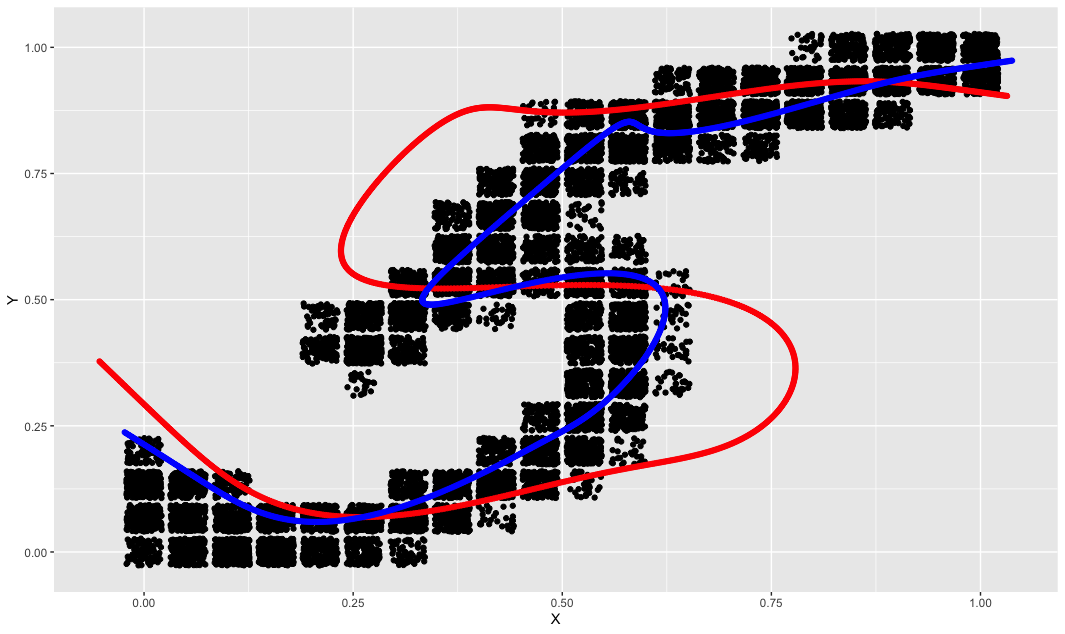
\includegraphics[width=9cm]{mnist_5plot1}}}%
  \hfill
  \subfloat[\centering MNIST Image 2]{{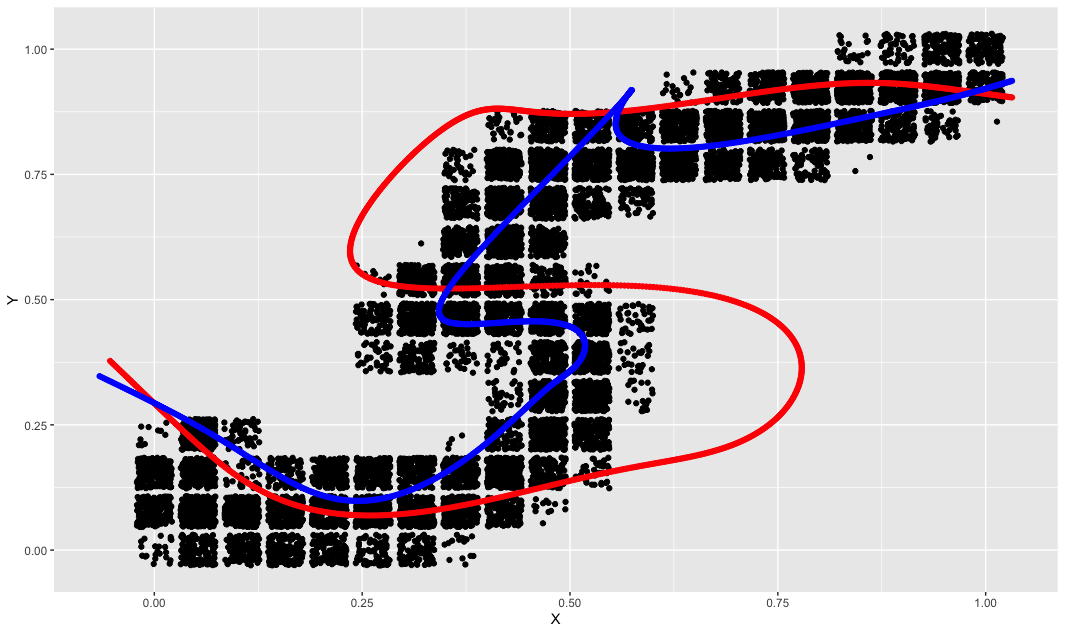
\includegraphics[width=9cm]{mnist_5plot2}}}
  \vfill
  \subfloat[\centering MNIST Image 3]{{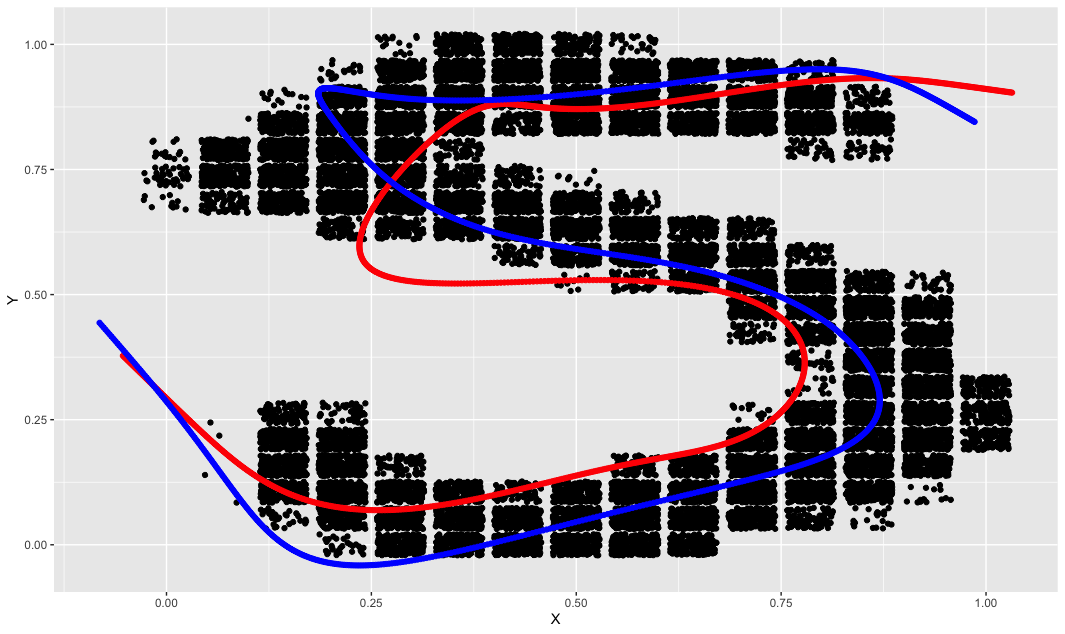
\includegraphics[width=9cm]{mnist_5plot3}}}
  \hfill
  \subfloat[\centering MNIST Image 4]{{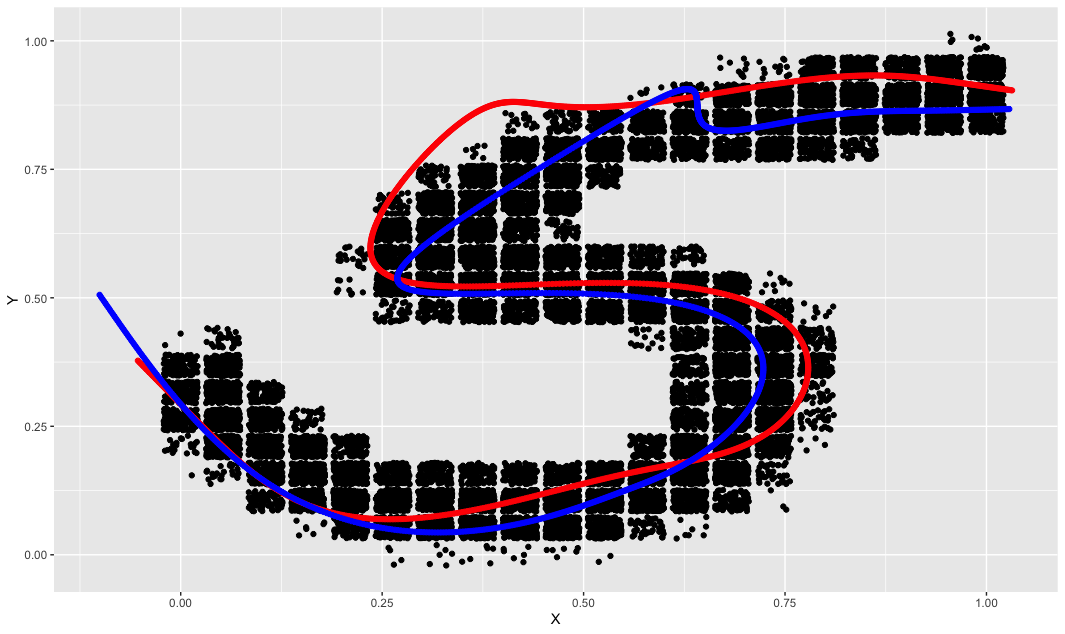
\includegraphics[width=9cm]{mnist_5plot4}}}
  \caption{Comparison of PME, Population, and Image-Level Results for MNIST Data}
  \label{fig:mnist_results}
\end{figure}

\section{Proposed Work} \label{s:hpme_adni}
Further work will be dedicated to testing the proposed approach in several settings. First, more extensive performance comparisons between the PME algorithm and its hierarchical extension will be conducted when applied to the MNIST dataset. The method will next be applied to a series of simulated datasets that were generated to reflect the hierarchical structure present in the ADNI dataset. Again, the estimates of the hierarchical approach will be compared to alternative methods, with the fit of each method to the data being compared. Finally, the hierarchical approach will be applied to structural MRI data from the ADNI dataset. Specifically, the algorithm can be used to estimate the manifolds underlying the hippocampus of study participants. Of interest in this case will be a comparison of the varying-coefficient models by group, which may provide a visual confirmation that the algorithm's estimates are detecting the most relevant information included in the data.

\newpage

\bibliographystyle{jasa}
\bibliography{references}


\end{document}
